\chapter{Esperimenti}

\section{Primi Classificatori}
\label{par:primi-classificatori}
Come discusso nel Capitolo \ref{ch:flf}, possiamo trattare tutti i modelli di un FLF che precedono l'ultimo in maniera omogenea. In questo paragrafo, presentiamo i due approcci che abbiamo esplorato in merito a questi primi classificatori.






\subsection{SVM Lineari}
\label{par:exp-svm}
Come prima strategia, abbiamo impiegato delle SVM Lineari (illustrate nel Paragrafo \ref{par:svm}). Il vantaggio di questo modello risiede nello spazio che occupa, che è piccolo e costante. Infatti, assumendo che ogni numero sia rappresentato su 32 bit, la dimensione di ciascuna SVM $m_j$ è pari a $b = (d+1) \cdot 32$ bit, dove $d$ è il numero di attributi nel dataset. Questo perché ciascun $m_j$ non è altro che un iperpiano, e dunque ha un coefficiente per ogni dimensione e un termine noto.

Un'altra importante proprietà delle SVM Lineari è data dalla presenza degli iperparametri $C_+$ e $C_-$, che permettono di regolare ciascun $\epsilon_j$, ossia il FPR empirico del modello $m_j$. Come già sottolineato nel Paragrafo \ref{par:fpr-flf}, poter regolare gli $\epsilon_j$ è fondamentale per avere controllo su $\epsilon$, il FPR complessivo del FLF. Da qui in avanti, ci riferiamo alla coppia $C_+, C_-$ per indicare specificatamente $C_+$ e $C_-$ della $j$-esima SVM, ossia di $m_j$

Riprendendo gli Algoritmi \ref{alg:addestramento-catena-completo-1} e \ref{alg:addestramento-catena-completo-2}, consideriamo una singola iterazione. Abbiamo dunque un train set $A_j$, un test set $T_j$ e un FPR $z$ a cui $\epsilon_j$ deve tendere (possibilmente standovi al sotto). 

A tale scopo, l'idea è fissare $C_- = 1$ e far variare solo $C_+$ per modulare il FPR di $m_j$. Come già illustrato, sempre nel Paragrafo \ref{par:svm}, aumentare $C_+$ porta a un aumento del FPR; diminuire $C_+$, invece, ne provoca una diminuzione. Dal momento che $C_+$ influenza in maniera monotonica crescente $\epsilon_j$, possiamo sfruttare una ricerca dicotomica su un dato intervallo di valori di $C_+$ per trovare quello che genera un $\epsilon_j$ il più vicino possibile a $z$.
A ogni iterazione $l$ della ricerca dicotomica, utilizziamo per $C_+^{(l)}$ il valore centrale dell'intervallo corrente, calcoliamo $\epsilon_j^{(l)}$ su $T_j$ e lo confrontiamo con $z$. Se si ha $\epsilon_j^{(l)} > z$, allora $C_+^{(l)}$ è troppo alto, e la ricerca va proseguita nella metà inferiore dell'intervallo. Se, invece, si ha $\epsilon_j^{(l)} < z$, allora si prosegue nella metà superiore. Nel caso improbabile in cui $\epsilon_j^{(l)} = z$, la ricerca termina.
Nella quasi totalità dei casi, il processo termina quando l'ampiezza dell'intervallo di ricerca scende sotto una data soglia $\delta$, prossima allo 0.
L'Algoritmo \ref{alg:addestramento-svm} illustra l'addestramento della $j$-esima SVM.

\begin{algorithm}
    \caption{Addestramento della SVM $j$-esima}
    \begin{algorithmic}[1]
        \Require $A_j$, $T_j$, $z, C_+^{\text{min}}, C_+^{\text{max}}, \delta$
        \Ensure $m_j$, $\epsilon_j$
        \State $C_- \gets 1$
        \While {$C_+^{\text{max}}-C_+^{\text{min}} \geq \delta$}
            \State $C_+ \gets (C_+^{\text{min}}+C_+^{\text{max}})/2$
            \State Addestra una SVM $m_j$ con $C_+, C_-$ su $A_j$
            \State $\epsilon_j \gets |\{(\mathbf{x}_i, y_i) \in T_j \enspace | \enspace m_j(\mathbf{x}_i) = 1 \}|/|T_j|$

            \If{$\epsilon_j > z$}
                \State $C_+^{\text{max}} \gets C_+$
            \ElsIf{$\epsilon_j < z$}
                \State $C_+^{\text{min}} \gets C_+$
            \Else
                \State \Return $m_j, \epsilon_j$
            \EndIf
            
        \EndWhile
        \State \Return $m_j, \epsilon_j$
    \end{algorithmic}
    \label{alg:addestramento-svm}
\end{algorithm}








\subsection{Reti Neurali}
\label{par:addestramento-nn}
In un secondo approccio, abbiamo utilizzato delle NN, presentate nel Paragrafo \ref{par:nn}. Come già evidenziato nel suddetto paragrafo, poter stabilire la topologia di rete è un grande vantaggio delle NN, in quanto permette di regolarne l'espressività. 
Nel nostro caso, vogliamo trovare la rete $m_j$ con topologia minima (ossia, col minor numero di neuroni) che, allenata su $A_j$, abbia un $\epsilon_j$ tale che $|\epsilon_j - z| \leq \sigma$ ($\sigma$, ricordiamo, è una soglia di precisione, iperparametro del FLF).
Chiaramente, dalla topologia di $m_j$ deriva lo spazio occupato $b_j$. In particolare, se abbiamo una rete con $G$ livelli (escludendo lo strato di input), dove il livello $g$-esimo ha $r$ neuroni, il numero totale $\Omega$ di parametri è
\begin{equation}
    \Omega = \sum_{g=1}^{G} (r_g \cdot r_{g-1} + r_g) \enspace,
\end{equation}
dove:
\begin{itemize}
    \item $r_g \cdot r_{g-1}$ rappresenta il numero di pesi che collegano il livello $g-1$ al livello $g$,
    \item $r_g$ rappresenta il numero di bias del livello $g$ (uno per ogni neurone).
\end{itemize}
Rappresentando ogni numero su 32 bit, possiamo dunque affermare che $b_j = \Omega_j \cdot 32$ bit, dove $\Omega_j$ è il numero di parametri della NN $m_j$. 
Chiaramente, non siamo più in uno scenario come quello relativo alle SVM lineari, in cui ciascun $m_j$ occupa uno spazio piccolo e costante.

La ricerca della topologia minima per ciascun $m_j$ riguarda in realtà solo gli strati nascosti: non abbiamo controllo su quello di input, che dipende dal numero di attributi dei dati, né su quello di output, che, come già discusso, nel nostro caso contiene un solo neurone. Per semplificare, abbiamo scelto di considerare solo NN con 2 strati nascosti, ciascuno avente dimensione minima e massima rispettivamente di $H_{\text{min}}$ e $H_{\text{max}}$ neuroni.

Tale ricerca è svolta in maniera lineare, partendo da una rete avente $H_{\text{min}}$ neuroni per strato nascosto. A ogni iterazione:
\begin{enumerate}
    \item considerando la topologia corrente, con $H$ neuroni per strato nascosto, si esegue una ricerca dicotomica sull'iperparametro $C_+$ (descritto nel Paragrafo \ref{par:nn}) per trovare la rete con $\epsilon_j$ ottimo, esattamente con gli stessi fini e modalità relativi alle SVM, come descritto nel Paragrafo \ref{par:exp-svm};
    \item se la rete trovata al punto 1 è tale che $|\epsilon_j - z| \leq \sigma$, la ricerca termina; altrimenti, se $H < H_{\text{max}}$, si incrementa $H$ di 1 e si torna al punto 1.
\end{enumerate}

L'Algoritmo \ref{alg:addestramento-nn} illustra il processo completo col quale si ricavano $m_j$ e $\epsilon_j$.

\begin{algorithm}[ht]
    \caption{Addestramento della NN $j$-esima}
    \begin{algorithmic}[1]
        \Require $A_j$, $T_j$, $z, \delta, \sigma, C_+^{\text{min}}, C_+^{\text{max}}, H_{\text{min}}, H_{\text{max}}$
        \Ensure $m_j$, $\epsilon_j$
        \State $C_- \gets 1$
        \For{$H$ in $H_{\text{min}}, \dots H_{\text{max}}$}
            \State $C_+^{\text{inf}} \gets C_+^{\text{min}}$
            \State $C_+^{\text{sup}} \gets C_+^{\text{max}}$

            \While {$C_+^{\text{sup}}-C_+^{\text{inf}} \geq \delta$}
                \State $C_+ \gets (C_+^{\text{inf}}+C_+^{\text{sup}})/2$
                \State Addestra su $A_j$ una NN $m_j$ con $C_+, C_-$ e $H$ neuroni per strato nascosto
                \State $\epsilon_j \gets |\{(\mathbf{x}_i, y_i) \in T_j \enspace | \enspace m_j(\mathbf{x}_i) = 1 \}|/|T_j|$
    
                \If{$\epsilon_j > z$}
                    \State $C_+^{\text{sup}} \gets C_+$
                \ElsIf{$\epsilon_j < z$}
                    \State $C_+^{\text{inf}} \gets C_+$
                \Else
                    \State \textbf{break}
                \EndIf
            \EndWhile

            \If{$|\epsilon_j - z| \leq \sigma$}
                \State \Return $m_j, \epsilon_j$
            \EndIf
            
        \EndFor
        
        \State \Return $m_j, \epsilon_j$ \Comment{Non è stata trovata alcuna NN, tra quelle possibili, in grado di raggiungere un FPR ammissibile. Restituiamo comunque $m_j, \epsilon_j$.}
    \end{algorithmic}
    \label{alg:addestramento-nn}
\end{algorithm}







\section{Ultimo Classificatore}
\label{par:ultimo-classificatore}
Come ultimo classificatore, abbiamo scelto di utilizzare un albero di decisione (Paragrafo \ref{par:dt}). Le motivazioni a supporto di questa scelta sono le seguenti.
Innanzitutto, esattamente come per le SVM lineari e le NN, abbiamo a disposizione gli iperparametri $C_+$ e $C_-$ per regolare il FPR e il FNR del modello. In secondo luogo, questa tipologia di modello è particolarmente predisposta a fare overfitting sul train set, che, come abbiamo esposto nel Paragrafo \ref{par:ultima-iterazione} è un requisito essenziale per l'ultimo classificatore di un FLF.

L'obiettivo è trovare il DT $m_j$ di dimensione minima tale che $\epsilon_j \leq z$ e che il FNR su $A_j$, che indichiamo come $\text{FNR}_{A_j}$, sia nullo; ossia, che trovi tutte le chiavi rimaste in $A_j$.
Fissata una dimensione massima per il DT attraverso l'iperparametro $F$, che determina il massimo numero di foglie generabili, vogliamo trovare il più piccolo valore di $C_+$ che garantisca $\text{FNR}_{A_j}=0$. Questo perché, come sappiamo, $\epsilon_j$ aumenta con $C_+$; dunque, stiamo sostanzialmente cercando, fissata una dimensione massima, l'albero con $\text{FNR}_{A_j}=0$ che abbia $\epsilon_j$ minimo. A tale scopo, definiamo un insieme ordinato $\Gamma$ di valori per $C_+$, ed eseguiamo una scansione lineare su di esso che termina quando il DT addestrato con il valore di $C_+$ corrente ottiene $\text{FNR}_{A_j}=0$. Se ciò non si verifica per nessun valore di $C_+ \in \Gamma$, allora è necessario incrementare $F$, se possibile.
Di fatto, questa ricerca lineare su $C_+$ viene annidata all'interno di una ricerca dicotomica su $F$ in un intervallo discreto $[F_{\text{min}}, F_{\text{max}}]$, nell'idea che DT di dimensioni maggiori producano sempre risultati migliori rispetto a quelli più piccoli (o almeno, questo è ciò che ci si aspetta). In questo modo, dovremmo trovare il DT di dimensione minima che abbia $\epsilon_j \leq z$ e $\text{FNR}_{A_j}=0$. Da notare che $F_{\text{max}}$, nel contesto dell'Algoritmo \ref{alg:addestramento-catena-completo-1}, assume il valore di $b_{\text{max}}$, ossia dello spazio disponibile rimasto.

L’Algoritmo \ref{alg:addestramento-dt} illustra lo schema col quale si ricava il DT $m_j$ e il relativo FPR empirico $\epsilon_j$.

\begin{algorithm}[ht]
    \caption{Addestramento del DT}
    \begin{algorithmic}[1]
        \Require $A_j$, $T_j$, $z, \delta_1, \delta_2, \Gamma, F_{\text{min}}, F_{\text{max}}$
        \Ensure $m_j$, $\epsilon_j$
        \State $C_- \gets 1$
        \State $m_j^* \gets $ \textbf{Null}
        \State $\epsilon_j^* \gets 1$
        
        \While{$F_{\text{min}} \leq F_{\text{max}}$}
            \State $F \gets \lfloor (F_{\text{min}} + F_{\text{max}})/2 \rfloor$
    
            \For {$C_+ \in \Gamma$}
                \State Addestra su $A_j$ un DT $m_j$ con $C_+, C_-$ e al massimo $F$ foglie
                \State $\epsilon_j \gets |\{(\mathbf{x}_i, y_i) \in T_j \enspace | \enspace m_j(\mathbf{x}_i) = 1 \}|/|T_j|$
    
                \If{$\text{FNR}_{A_j} = 0$}
                    \State \textbf{break}
                \EndIf
            \EndFor

            \If{$\epsilon_j \leq z$ \textbf{and} $\text{FNR}_{A_j} = 0$}
                \State $m_j^* \gets m_j$
                \State $\epsilon_j^* \gets \epsilon_j$
                \State $F_{\text{max}} \gets F+1$
            \Else
                \State $F_{\text{min}} \gets F-1$
            \EndIf
            
        \EndWhile
        
        \State \Return $m_j^*, \epsilon_j^*$ \Comment{NB: si potrebbe arrivare a questa istruzione avendo ancora $m_j^* =$ Null e $\epsilon_j^* = 1$.}
    \end{algorithmic}
    \label{alg:addestramento-dt}
\end{algorithm}











\section{Risultati}
Gli esperimenti sono stati condotti su cinque dataset, generati utilizzando la la funzione \texttt{make\_classification}, implementata nella libreria \textit{scikit-learn}.
Questa funzione genera dataset sintetici mediante la creazione di cluster gaussiani e l'introduzione controllata di rumore.
Facendo variare solamente il parametro \texttt{class\_sep} per avvicinare i cluster di esempi positivi e negativi, abbiamo ottenuto dataset di difficoltà crescente.
Ciascun dataset di partenza contiene 20296 chiavi e 55792 non-chiavi. 23912 di queste ultime fanno parte del relativo train set, insieme alle chiavi, mentre le restanti costituiscono il test set. Inoltre, ogni dataset è composto da osservazioni bidimensionali, il che ci permette di visualizzarli facilmente nel piano cartesiano. Le Figure \ref{fig:ds1} e \ref{fig:ds5} mostrano i train set 1 e 5.

\begin{table}[h]
    \centering
    \begin{tabular}{|c|c|c|}
        \hline
        Dataset & \texttt{class\_sep} & $\mathrm{F1v}$ \\
        \hline
        1 & 0.1 & 0.05 \\
        2 & 0.3 & 0.10 \\
        3 & 0.5 & 0.31 \\
        4 & 1.0 & 0.56 \\
        5 & 1.5 & 0.92 \\
        \hline
    \end{tabular}
    \caption{Valori del parametro \texttt{class\_sep} utilizzati nella generazione e score sulla metrica $\mathrm{F1v}$ per ognuno dei cinque dataset considerati.}
    \label{tab:datasets}
\end{table}


\begin{figure}[h!]
    \centering
    \begin{minipage}{0.49\textwidth}
        \centering
        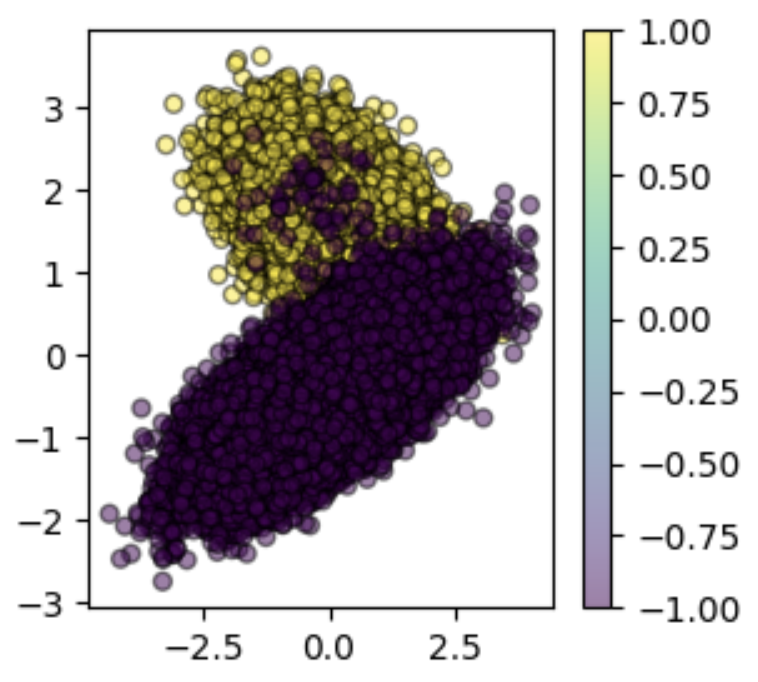
\includegraphics[width=\linewidth]{images/ds1.png}
        \caption{Train set 1.}
        \label{fig:ds1}
    \end{minipage}
    \hfill
    \begin{minipage}{0.49\textwidth}
        \centering
        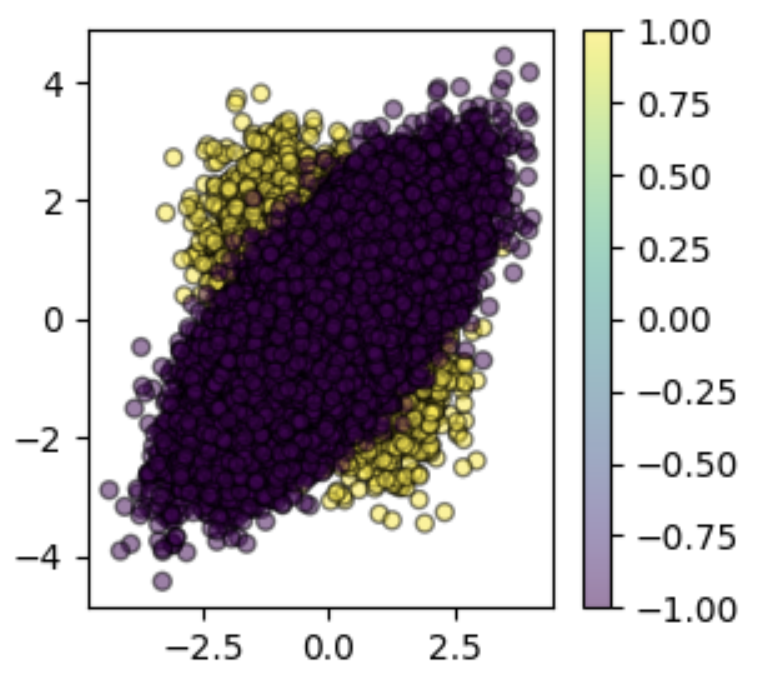
\includegraphics[width=\linewidth]{images/ds5.png}
        \caption{Train set 5.}
        \label{fig:ds5}
    \end{minipage}
\end{figure}

Di seguito, elenchiamo i valori di alcuni iperparametri rimasti immutati per tutti gli esperimenti. La simbologia adottata è la stessa rispetto ai Paragrafi \ref{par:primi-classificatori} e \ref{par:ultimo-classificatore}.
\begin{itemize}
    \item $C_+^{\text{min}} = 0.01, C_+^{\text{max}}=20$;

    \item $\Gamma$ contiene i valori da 0.1 a 50 con incrementi di 0.1;

    \item $H_{\text{min}} = 1, H_{\text{max}}=50$;

    \item $\sigma = 0.3z$;

    \item $F_{\text{min}} = 1$.
\end{itemize}











\subsection{SVM}
\label{par:svm-results}

Le Tabelle \ref{tab:performance-ds1-svm}-\ref{tab:performance-ds5-svm} illustrano le performance di vari FLF, addestrati usando SVM lineari, sui dataset considerati. In ciascuna tabella le colonne, in ordine, sono:
\begin{itemize}
    \item la lunghezza massima della catena ($t$),
    \item il FPR richiesto ($\bar \epsilon$),
    \item il numero di classificatori effettivamente impiegati,
    \item il FPR empirico raggiunto sul test set,
    \item il rapporto, in percentuale, tra lo spazio occupato dalla catena e quello occupato da un BF classico che gestisce lo stesso numero di chiavi con lo stesso FPR empirico.
\end{itemize}
In ogni tabella, ciascuna riga si riferisce a una specifica combinazione di $t$ e $\bar \epsilon$, che sono iperparametri. Il segno * indica che, per la relativa combinazione di $t$ e $\bar \epsilon$, l'addestramento ha portato ad avere solo un DT, senza alcuna SVM prima di esso.

È importante precisare che in nessun caso utilizzare un albero di decisione come ultimo classificatore della catena è stato conveniente rispetto a impiegare un BF classico.












La Tabella \ref{tab:svm-skip} prende in considerazione una singola catena avente $t=20$ e $\bar\epsilon=0.1$ e illustra l'andamento di alcuni dati rilevanti al proseguire delle iterazioni (indicizzate con $j$) durante l'addestramento di un FLF sul dataset 1, quello più semplice. I dati riportati sono:
\begin{itemize}
\item le chiavi rimaste al termine dell'iterazione $j$-esima,
\item le non-chiavi rimaste al termine dell'iterazione $j$-esima,
\item il FPR empirico del classificatore $j$-esimo,
\item il valore di $z$ per il classificatore $j$-esimo,
\item lo spazio, in bit, occupato dal classificatore $j$-esimo,
\item il rapporto, in percentuale, tra lo spazio occupato dal classificatore e quello occupato dal BF classico equivalente (indicato con $\rho$).
\end{itemize}

La Tabella \ref{tab:svm-no-skip} è analoga alla Tabella \ref{tab:svm-skip}, ma riguarda un setting in cui non è possibile effettuare salti all'ultimo classificatore, permettendo l'aggiunta anche di modelli sconvenienti dal punto di vista dello spazio.















\subsection{NN}

Le Tabelle \ref{tab:performance-ds1-mlp}-\ref{tab:performance-ds5-mlp} sono analoghe a quelle del Paragrafo \ref{par:svm-results}, ma si riferiscono a uno scenario in cui il FLF impiega NN al posto di SVM lineari.
Anche in questo caso, utilizzare un albero di decisione come ultimo classificatore della catena è sempre stato sconveniente rispetto a impiegare un BF classico.
Le Tabelle \ref{tab:mlp-skip} e \ref{tab:mlp-no-skip} sono rispettivamente analoghe alle Tabelle \ref{tab:svm-skip} e \ref{tab:svm-no-skip}, ma riguardano FLF che utilizzano NN.
















\subsection{Osservazioni}

Innanzitutto, è importante evidenziare che in nessun caso è stato conveniente utilizzare un DT come ultimo classificatore. Ciò significa che nessuno dei filtri ottenuti è puramente appreso; al contrario, ciascuno adotta un BF classico. Molto probabilmente questo è dovuto al fatto che, come osservato nel Paragrafo \ref{par:ultima-iterazione}, al progredire delle iterazioni, le chiavi che rimangono sono quelle più difficili da identificare, per cui il vantaggio di un modello di ML rispetto a un BF classico si fa via via più sottile. All'ultima iterazione, evidentemente, rimangono solo chiavi che non seguono alcun pattern, e dunque sfruttare un modello di ML perde di senso.

È da sottolineare anche il fatto che, fissato un $\bar \epsilon$, all'aumentare di $t$ l'efficienza tende, nella maggior parte dei casi, a peggiorare. Solitamente, i risultati migliori si hanno per $t=2$.

Tuttavia, nel complesso, un filtro basato su NN è quasi sempre più efficiente rispetto all'equivalente BF classico. Come ci sarebbe potuto aspettare, il vantaggio di questo tipo di filtro è minore su dataset in cui molte chiavi sono sovrapposte alle non-chiavi. Infatti, maggiore la sovrapposizione dei cluster di positivi e di negativi, maggiore è il rapporto tra lo spazio occupato dal filtro e da un BF classico. Sui dataset 4 e 5, per diverse combinazioni di $t$ e $\bar \epsilon$, tale rapporto arriva a essere maggiore di 1.

Confrontando i FLF basati su SVM con quelli basati su NN, notiamo che questi ultimi tendono a essere più efficienti, specialmente all'aumentare della difficoltà del dataset.
È importante sottolineare, però, che abbiamo considerato solo dataset formati da un cluster per classe; se ce ne fossero stati ulteriori, il problema sarebbe stato meno lineare e dunque più difficile per le SVM lineari.

Sul dataset 5, con i FLF basati su SVM, emerge un comportamento del filtro che differisce da quello osservato sui dataset precedenti. Data la grande difficoltà del dataset, se $t$ supera un certo valore, la seconda SVM non riesce a raggiungere il FPR richiesto (che diventa più stringente all'aumentare di $t$); dunque, si salta all'ultimo classificatore, il BF classico, dopo una sola iterazione. Si ottiene quindi un filtro composto da una SVM, che riconosce pochi positivi, e da un BF classico che gestisce i restanti, ossia la quasi totalità delle chiavi. Per questo, i filtri così generati hanno dimensioni molto simili rispetto ai BF classici equivalenti.

Esaminando le tabelle che illustrano la progressione delle iterazioni di un singolo filtro, possiamo chiaramente notare l'impatto sull'efficienza della possibilità di effettuare il salto all'ultimo classificatore. 
Notiamo anche che $\rho$ tende ad aumentare nel corso delle iterazioni, con diminuzioni occasionali probabilmente dovute al fatto che alcuni modelli, commettendo FP, rimuovono anche alcune non-chiavi che ostacolavano particolarmente l'identificazione dei positivi.
È interessante notare anche che, nel caso del filtro basato su NN con possibilità di salto, le singole NN non hanno mai raggiunto grandi dimensioni; anzi, si sono mantenute tutte sulla dimensione minima (corrispondente a 1 neurone per strato nascosto). Quindi, anche con NN così piccole si può raggiungere il FPR accettabile.

\begin{table}
    \centering
    \begin{tabular}{|c|c|c|c|c|}
        \hline
        $t$ & $\bar\epsilon$ & Classificatori usati & $\epsilon$ empirico & Spazio rispetto a BF \\ 
        \hline
        2 & 0.1 & 2 & 0.109 & 3.13\% \\  
        3 & 0.1 & 3 & 0.105 & 3.44\% \\  
        4 & 0.1 & 4 & 0.106 & 3.75\% \\  
        5 & 0.1 & 5 & 0.104 & 4.07\% \\  
        10 & 0.1 & 8 & 0.107 & 4.00\% \\ 
        20 & 0.1 & 13 & 0.099 & 4.40\% \\ 
        50 & 0.1 & 22 & 0.101 & 5.20\% \\ 
        100 & 0.1 & * & * & * \\ 
        2 & 0.05 & 2 & 0.048 & 3.92\% \\  
        3 & 0.05 & 3 & 0.053 & 3.98\% \\  
        4 & 0.05 & 4 & 0.054 & 4.09\% \\  
        5 & 0.05 & 5 & 0.054 & 4.32\% \\  
        10 & 0.05 & 10 & 0.055 & 5.13\% \\ 
        20 & 0.05 & 19 & 0.056 & 5.79\% \\ 
        50 & 0.05 & * & * & * \\ 
        100 & 0.05 & * & * & * \\  
        \hline
    \end{tabular}
    \caption{Performance del filtro basato su SVM sul dataset 1.}
    \label{tab:performance-ds1-svm}
\end{table}
\begin{table}
    \centering
    \begin{tabular}{|c|c|c|c|c|}
        \hline
        $t$ & $\bar\epsilon$ & Classificatori usati & $\epsilon$ empirico & Spazio rispetto a BF \\ 
        \hline
        2  & 0.1  & 2  & 0.102 & 14.99\% \\  
        3  & 0.1  & 3  & 0.106 & 15.86\% \\  
        4  & 0.1  & 4  & 0.103 & 16.17\% \\  
        5  & 0.1  & 5  & 0.103 & 16.86\% \\  
        10 & 0.1  & 10 & 0.104 & 19.10\% \\ 
        20 & 0.1  & 20 & 0.102 & 22.32\% \\ 
        50 & 0.1  & 50 & 0.104 & 28.18\% \\ 
        100 & 0.1 & 82 & 0.103 & 24.80\% \\  
        2  & 0.05 & 2  & 0.050 & 20.32\% \\  
        3  & 0.05 & 3  & 0.052 & 21.24\% \\  
        4  & 0.05 & 4  & 0.051 & 21.74\% \\  
        5  & 0.05 & 5  & 0.052 & 22.62\% \\  
        10 & 0.05 & 10 & 0.054 & 25.17\% \\ 
        20 & 0.05 & 20 & 0.053 & 28.86\% \\ 
        50 & 0.05 & 50 & 0.054 & 34.42\% \\ 
        100 & 0.05 & *  & *     & *      \\  
        \hline
    \end{tabular}
    \caption{Performance del filtro basato su SVM sul dataset 2.}
    \label{tab:performance-ds2-svm}
\end{table}
\begin{table}
    \centering
    \begin{tabular}{|c|c|c|c|c|}
        \hline
        $t$ & $\bar\epsilon$ & Classificatori usati & $\epsilon$ empirico & Spazio rispetto a BF \\ 
        \hline
        2  & 0.1  & 2  & 0.102 & 62.29\% \\  
        3  & 0.1  & 3  & 0.107 & 73.57\% \\  
        4  & 0.1  & 4  & 0.106 & 79.50\% \\  
        5  & 0.1  & 5  & 0.104 & 83.96\% \\  
        10 & 0.1  & 10 & 0.105 & 97.19\% \\ 
        20 & 0.1  & 20 & 0.105 & 112.48\% \\ 
        50 & 0.1  & 50 & 0.104 & 135.49\% \\ 
        100 & 0.1 & 51 & 0.105 & 76.90\% \\  
        2  & 0.05 & 2  & 0.053 & 68.94\% \\  
        3  & 0.05 & 3  & 0.055 & 78.91\% \\  
        4  & 0.05 & 4  & 0.054 & 83.89\% \\  
        5  & 0.05 & 5  & 0.053 & 87.94\% \\  
        10 & 0.05 & 10 & 0.053 & 100.69\% \\ 
        20 & 0.05 & 20 & 0.053 & 112.59\% \\ 
        50 & 0.05 & 50 & 0.053 & 132.77\% \\ 
        100 & 0.05 & 39 & 0.052 & 77.14\% \\  
        \hline
    \end{tabular}
    \caption{Performance del filtro basato su SVM sul dataset 3.}
    \label{tab:performance-ds3-svm}
\end{table}
\begin{table}
    \centering
    \begin{tabular}{|c|c|c|c|c|}
        \hline
        $t$ & $\bar\epsilon$ & Classificatori usati & $\epsilon$ empirico & Spazio rispetto a BF \\ 
        \hline
        2  & 0.1  & 2  & 0.101 & 85.31\% \\  
        3  & 0.1  & 3  & 0.108 & 101.83\% \\  
        4  & 0.1  & 4  & 0.104 & 112.89\% \\  
        5  & 0.1  & 5  & 0.106 & 120.41\% \\  
        10 & 0.1  & 10 & 0.104 & 143.40\% \\ 
        20 & 0.1  & 20 & 0.103 & 165.85\% \\ 
        50 & 0.1  & 50 & 0.104 & 195.58\% \\ 
        100 & 0.1 & 20 & 0.103 & 90.63\% \\  
        2  & 0.05 & 2  & 0.051 & 89.88\% \\  
        3  & 0.05 & 3  & 0.052 & 103.12\% \\  
        4  & 0.05 & 4  & 0.053 & 112.02\% \\  
        5  & 0.05 & 5  & 0.052 & 118.67\% \\  
        10 & 0.05 & 10 & 0.054 & 135.93\% \\ 
        20 & 0.05 & 20 & 0.053 & 155.21\% \\ 
        50 & 0.05 & 28 & 0.052 & 102.28\% \\ 
        100 & 0.05 & 13 & 0.050 & 91.15\% \\  
        \hline
    \end{tabular}
    \caption{Performance del filtro basato su SVM sul dataset 4.}
    \label{tab:performance-ds4-svm}
\end{table}
\begin{table}
    \centering
    \begin{tabular}{|c|c|c|c|c|}
        \hline
        $t$ & $\bar\epsilon$ & Classificatori usati & $\epsilon$ empirico & Spazio rispetto a BF \\ 
        \hline
        2  & 0.1  & 2  & 0.107 & 106.23\% \\  
        3  & 0.1  & 3  & 0.104 & 125.15\% \\  
        4  & 0.1  & 4  & 0.101 & 138.85\% \\  
        5  & 0.1  & 2  & 0.098 & 97.27\% \\  
        10 & 0.1  & 2  & 0.104 & 96.11\% \\ 
        20 & 0.1  & 2  & 0.098 & 96.13\% \\ 
        50 & 0.1  & 2  & 0.100 & 96.58\% \\ 
        100 & 0.1 & 2  & 0.105 & 97.06\% \\  
        2  & 0.05 & 2  & 0.052 & 107.82\% \\  
        3  & 0.05 & 2  & 0.049 & 102.24\% \\  
        4  & 0.05 & 2  & 0.050 & 99.98\% \\  
        5  & 0.05 & 2  & 0.052 & 98.98\% \\  
        10 & 0.05 & 2  & 0.049 & 97.40\% \\ 
        20 & 0.05 & 2  & 0.050 & 97.16\% \\ 
        50 & 0.05 & 2  & 0.049 & 97.30\% \\ 
        100 & 0.05 & 2  & 0.051 & 97.95\% \\  
        \hline
    \end{tabular}
    \caption{Performance del filtro basato su SVM sul dataset 5.}
    \label{tab:performance-ds5-svm}
\end{table}
\begin{table}
\centering
\begin{tabular}{|c|c|c|c|c|c|c|}
\hline
$j$ & Chiavi & Non-chiavi & $\epsilon_i \cdot 10^2$ & $z_i \cdot 10^2$ & Spazio [bit] & $\rho$ [\%] \\
\hline
1 & 1198 & 55495 & 0.5269 & 0.5254 & 96 & 0.05 \\
2 & 935 & 55219 & 0.5213 & 0.5253 & 96 & 3.34 \\
3 & 785 & 54929 & 0.5240 & 0.5256 & 96 & 5.85 \\
4 & 696 & 54642 & 0.5268 & 0.5257 & 96 & 9.88 \\
5 & 634 & 54380 & 0.5211 & 0.5256 & 96 & 14.14 \\
6 & 591 & 54042 & 0.5324 & 0.5259 & 96 & 20.47 \\
7 & 545 & 53739 & 0.5180 & 0.5254 & 96 & 19.05 \\
8 & 524 & 53372 & 0.5380 & 0.5260 & 96 & 41.92 \\
9 & 508 & 53111 & 0.5235 & 0.5250 & 96 & 54.86 \\
10 & 495 & 52813 & 0.5262 & 0.5251 & 96 & 67.61 \\
11 & 484 & 52557 & 0.5290 & 0.5250 & 96 & 79.34 \\
12 & 471 & 52323 & 0.5230 & 0.5246 & 96 & 67.13 \\
13 & 0 & 50260 & 4.072 & 4.122 & 3126 & (100) \\
\hline
\end{tabular}
\caption{Progressione delle iterazioni utilizzando SVM lineari e con la possibilità di salto. FPR empirico: 0.099; spazio rispetto a un BF equivalente: 4.40\%.}
\label{tab:svm-skip}
\end{table}
\begin{table}
\centering
\begin{tabular}{|c|c|c|c|c|c|c|}
\hline
$j$ & Chiavi & Non-chiavi & $\epsilon_i \cdot 10^3$ & $z_i \cdot 10^3$ & Spazio [bit] & $\rho$ [\%] \\
\hline
1  & 1198  & 55495 & 5.269 & 5.254 & 96   & 0.05 \\
2  & 935   & 55219 & 5.213 & 5.253 & 96   & 3.34 \\
3  & 785   & 54929 & 5.240 & 5.256 & 96   & 5.85 \\
4  & 696   & 54642 & 5.268 & 5.257 & 96   & 9.88 \\
5  & 634   & 54380 & 5.211 & 5.256 & 96   & 14.14 \\
6  & 591   & 54042 & 5.324 & 5.259 & 96   & 20.47 \\
7  & 545   & 53739 & 5.180 & 5.254 & 96   & 19.05 \\
8  & 524   & 53372 & 5.380 & 5.260 & 96   & 41.92 \\
9  & 508   & 53111 & 5.235 & 5.250 & 96   & 54.86 \\
10 & 495   & 52813 & 5.262 & 5.251 & 96   & 67.61 \\
11 & 484   & 52557 & 5.290 & 5.250 & 96   & 79.34 \\
12 & 471   & 52323 & 5.230 & 5.246 & 96   & 67.13 \\
13 & 464   & 52081 & 5.168 & 5.248 & 96   & 124.68 \\
14 & 455   & 51768 & 5.195 & 5.259 & 96   & 96.97 \\
15 & 439   & 51483 & 5.222 & 5.270 & 96   & 54.86 \\
16 & 434   & 51238 & 5.249 & 5.279 & 96   & 174.55 \\
17 & 430   & 50965 & 5.277 & 5.287 & 96   & 218.18 \\
18 & 421   & 50620 & 5.214 & 5.290 & 96   & 96.97 \\
19 & 418   & 50367 & 5.241 & 5.329 & 96   & 290.91 \\
20 & 0     & 50052 & 6.008 & 5.416 & 4540 & (100) \\
\hline
\end{tabular}
\caption{Progressione delle iterazioni utilizzando SVM lineari e senza la possibilità di salto. FPR empirico: 0.103; spazio rispetto a un BF equivalente: 65.42\%.}
\label{tab:svm-no-skip}
\end{table}
\begin{table}
    \centering
    \begin{tabular}{|c|c|c|c|c|}
        \hline
        $t$  & $\bar\epsilon$ & Classificatori usati & $\epsilon$ empirico & Spazio rispetto a BF \\ 
        \hline
        2   & 0.1  & 2  & 0.103 & 3.31\% \\ 
        3   & 0.1  & 3  & 0.105 & 3.70\% \\ 
        4   & 0.1  & 4  & 0.103 & 4.20\% \\ 
        5   & 0.1  & 5  & 0.103 & 4.65\% \\  
        10  & 0.1  & 6  & 0.107 & 4.39\% \\  
        20  & 0.1  & 9  & 0.103 & 4.97\% \\  
        2   & 0.05 & 2  & 0.050 & 4.02\% \\ 
        3   & 0.05 & 3  & 0.056 & 4.17\% \\ 
        4   & 0.05 & 4  & 0.053 & 4.39\% \\ 
        5   & 0.05 & 5  & 0.054 & 4.72\% \\  
        10  & 0.05 & 8  & 0.049 & 5.21\% \\  
        20  & 0.05 & 10 & 0.054 & 5.50\% \\  
        \hline
    \end{tabular}
    \caption{Performance del filtro basato su NN sul dataset 1.}
    \label{tab:performance-ds1-mlp}
\end{table}
\begin{table}
    \centering
    \begin{tabular}{|c|c|c|c|c|}
        \hline
        $t$  & $\bar\epsilon$ & Classificatori usati & $\epsilon$ empirico & Spazio rispetto a BF \\ 
        \hline
        2   & 0.1  & 2  & 0.100 & 15.11\% \\ 
        3   & 0.1  & 3  & 0.106 & 16.66\% \\ 
        4   & 0.1  & 4  & 0.103 & 16.72\% \\ 
        5   & 0.1  & 5  & 0.104 & 17.43\% \\  
        10  & 0.1  & 10 & 0.102 & 20.78\% \\  
        20  & 0.1  & 20 & 0.105 & 26.58\% \\  
        2   & 0.05 & 2  & 0.049 & 20.39\% \\ 
        3   & 0.05 & 3  & 0.051 & 22.24\% \\ 
        4   & 0.05 & 4  & 0.052 & 22.12\% \\ 
        5   & 0.05 & 5  & 0.052 & 23.28\% \\  
        10  & 0.05 & 10 & 0.052 & 24.82\% \\  
        20  & 0.05 & 20 & 0.052 & 29.77\% \\  
        \hline
    \end{tabular}
    \caption{Performance del filtro basato su NN sul dataset 2.}
    \label{tab:performance-ds2-mlp}
\end{table}
\begin{table}
    \centering
    \begin{tabular}{|c|c|c|c|c|}
        \hline
        $t$  & $\bar\epsilon$ & Classificatori usati & $\epsilon$ empirico & Spazio rispetto a BF \\ 
        \hline
        2   & 0.1  & 2  & 0.106 & 62.68\% \\ 
        3   & 0.1  & 3  & 0.105 & 61.95\% \\ 
        4   & 0.1  & 4  & 0.098 & 63.90\% \\ 
        5   & 0.1  & 5  & 0.100 & 66.16\% \\  
        10  & 0.1  & 10 & 0.100 & 75.80\% \\  
        20  & 0.1  & 20 & 0.101 & 90.13\% \\  
        2   & 0.05 & 2  & 0.047 & 69.57\% \\ 
        3   & 0.05 & 3  & 0.049 & 68.86\% \\ 
        4   & 0.05 & 4  & 0.049 & 70.65\% \\ 
        5   & 0.05 & 5  & 0.050 & 73.69\% \\  
        10  & 0.05 & 10 & 0.049 & 85.20\% \\  
        20  & 0.05 & 20 & 0.049 & 94.67\% \\  
        \hline
    \end{tabular}
    \caption{Performance del filtro basato su NN sul dataset 3.}
    \label{tab:performance-ds3-mlp}
\end{table}
\begin{table}
    \centering
    \begin{tabular}{|c|c|c|c|c|}
        \hline
        $t$  & $\bar\epsilon$ & Classificatori usati & $\epsilon$ empirico & Spazio rispetto a BF \\ 
        \hline
        2   & 0.1  & 2  & 0.099 & 77.00\% \\ 
        3   & 0.1  & 3  & 0.099 & 83.31\% \\ 
        4   & 0.1  & 4  & 0.094 & 87.23\% \\ 
        5   & 0.1  & 5  & 0.098 & 92.26\% \\  
        10  & 0.1  & 10 & 0.098 & 108.26\% \\  
        20  & 0.1  & 20 & 0.097 & 123.45\% \\  
        2   & 0.05 & 2  & 0.052 & 81.85\% \\ 
        3   & 0.05 & 3  & 0.050 & 87.74\% \\ 
        4   & 0.05 & 4  & 0.049 & 92.05\% \\ 
        5   & 0.05 & 5  & 0.048 & 96.27\% \\  
        10  & 0.05 & 10 & 0.049 & 106.96\% \\  
        20  & 0.05 & 20 & 0.049 & 128.04\% \\  
        \hline
    \end{tabular}
    \caption{Performance del filtro basato su NN sul dataset 4.}
    \label{tab:performance-ds4-mlp}
\end{table}
\begin{table}
    \centering
    \begin{tabular}{|c|c|c|c|c|}
        \hline
        $t$  & $\bar\epsilon$ & Classificatori usati & $\epsilon$ empirico & Spazio rispetto a BF \\ 
        \hline
        2   & 0.1  & 2  & 0.095 & 95.15\% \\ 
        3   & 0.1  & 3  & 0.100 & 104.46\% \\ 
        4   & 0.1  & 4  & 0.096 & 111.72\% \\ 
        5   & 0.1  & 5  & 0.097 & 117.78\% \\  
        10  & 0.1  & 10 & 0.098 & 143.04\% \\  
        20  & 0.1  & 20 & 0.093 & 152.17\% \\  
        2   & 0.05 & 2  & 0.053 & 97.09\% \\ 
        3   & 0.05 & 3  & 0.050 & 106.45\% \\ 
        4   & 0.05 & 4  & 0.050 & 111.99\% \\ 
        5   & 0.05 & 5  & 0.050 & 117.11\% \\  
        10  & 0.05 & 10 & 0.046 & 127.85\% \\  
        20  & 0.05 & 20 & 0.047 & 147.61\% \\  
        \hline
    \end{tabular}
    \caption{Performance del filtro basato su NN sul dataset 5.}
    \label{tab:performance-ds5-mlp}
\end{table}
\begin{table}
\centering
\begin{tabular}{|c|c|c|c|c|c|c|}
\hline
$j$ & Chiavi & Non-chiavi & $\epsilon_i \cdot 10^3$ & $z_i \cdot 10^3$ & Spazio [bit] & $\rho$ [\%] \\
\hline
1 & 1201 & 55495 & 5.269 & 5.254 & 224 & 0.11 \\
2 & 931 & 55216 & 5.297 & 5.253 & 224 & 7.60 \\
3 & 783 & 54910 & 5.241 & 5.251 & 224 & 13.84 \\
4 & 698 & 54636 & 5.184 & 5.252 & 224 & 24.06 \\
5 & 636 & 54379 & 5.211 & 5.256 & 224 & 32.99 \\
6 & 599 & 54050 & 5.324 & 5.259 & 224 & 55.45 \\
7 & 552 & 53700 & 5.266 & 5.254 & 224 & 43.58 \\
8 & 524 & 53383 & 5.207 & 5.253 & 224 & 72.96 \\
9 & 0 & 50327 & 60.02 & 61.29 & 3045 & (100) \\
\hline
\end{tabular}
\caption{Progressione delle iterazioni utilizzando NN e con la possibilità di salto. FPR empirico: 0.103; spazio rispetto a un BF equivalente: 4.97\%.}
\label{tab:mlp-skip}
\end{table}
\begin{table}
\centering
\begin{tabular}{|c|c|c|c|c|c|c|}
\hline
$j$ & Chiavi & Non-chiavi & $\epsilon_i \cdot 10^3$ & $z_i \cdot 10^3$ & Spazio [bit] & $\rho$ [\%] \\
\hline
1  & 1201  & 55495 & 5.269 & 5.254 & 224  & 0.11 \\
2  & 931   & 55216 & 5.297 & 5.253 & 224  & 7.60 \\
3  & 783   & 54910 & 5.241 & 5.251 & 224  & 13.84 \\
4  & 698   & 54636 & 5.184 & 5.252 & 224  & 24.06 \\
5  & 636   & 54379 & 5.211 & 5.256 & 224  & 32.99 \\
6  & 599   & 54050 & 5.324 & 5.259 & 224  & 55.45 \\
7  & 552   & 53700 & 5.266 & 5.254 & 224  & 43.58 \\
8  & 524   & 53383 & 5.207 & 5.253 & 224  & 72.96 \\
9  & 494   & 53142 & 5.321 & 5.257 & 480  & 146.79 \\
10 & 474   & 52864 & 5.175 & 5.251 & 1184 & 538.18 \\
11 & 470   & 52644 & 5.113 & 5.259 & 1632 & 3709.09 \\
12 & 460   & 52284 & 5.140 & 5.275 & 480  & 436.36 \\
13 & 448   & 51980 & 5.166 & 5.292 & 1184 & 896.97 \\
14 & 438   & 51739 & 5.014 & 5.310 & 1184 & 1066.67 \\
15 & 430   & 51450 & 4.949 & 5.359 & 1184 & 1330.34 \\
16 & 422   & 51097 & 6.421 & 5.441 & 1184 & 1392.94 \\
17 & 420   & 50923 & 3.641 & 5.196 & 1184 & 4933.33 \\
18 & 417   & 50573 & 5.938 & 5.715 & 1632 & 4945.45 \\
19 & 414   & 50357 & 5.054 & 5.603 & 1632 & 4800.00 \\
20 & 0    & 50037 & 7.389 & 6.151 & 4386 & (100) \\
\hline
\end{tabular}
\caption{Progressione delle iterazioni utilizzando NN e senza la possibilità di salto. FPR empirico: 0.103; spazio rispetto a un BF equivalente: 19.67\%.}
\label{tab:mlp-no-skip}
\end{table}